\documentclass{article}
\usepackage{amsmath}
\usepackage{graphicx}
\usepackage{tikz}

\begin{document}

\begin{center}
    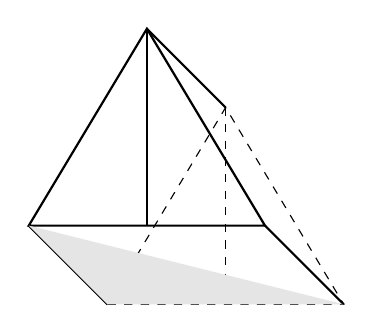
\begin{tikzpicture}

        % Draw the front triangular face (solid lines)
        \draw[thick] (0,0) -- (3,0) -- (1.5,2.5) -- cycle;

        % Draw the back triangular face (dashed lines)
        \draw[dashed] (1,-1) -- (4,-1) -- (2.5,1.5) -- cycle;

        % Connect the front and back faces with verticals
        \draw[thick] (0,0) -- (1,-1);  % bottom left edge (solid)
        \draw[thick] (3,0) -- (4,-1);  % bottom right edge (solid)
        \draw[thick] (1.5,2.5) -- (2.5,1.5);  % top edge (solid)

        % Vertical edges (dashed for the back)
        \draw[thick] (1.5,2.5) -- (1.5,0);  % front vertical (solid)
        \draw[dashed] (2.5,1.5) -- (2.5,-1);  % back vertical (dashed)
        \draw[dashed] (1,-1) -- (0,0);  % bottom back vertical (dashed)

        % Shade the bottom face
        \fill[gray!20] (1,-1) -- (4,-1) -- (0,0) -- cycle;

    \end{tikzpicture}

    \vspace{0.5cm}

    \textbf{Triangular Prism}

\end{center}

\end{document}
